\documentclass{../../slides-style}

\slidetitle{Деревья}{25.10.2023}

\begin{document}
    
    \begin{frame}[plain]
        \titlepage
    \end{frame}
    
    \begin{frame}
        \frametitle{Дерево}
        Ещё один абстрактный тип данных, используемый в программировании повсеместно
        \begin{columns}
            \begin{column}{0.55\textwidth}
                \begin{itemize}
                    \item Файловая система
                    \item Абстрактное синтаксическое дерево
                    \begin{itemize}
                        \item Дерево разбора арифметического выражения
                    \end{itemize}
                    \item Двоичное дерево поиска
                    \begin{itemize}
                        \item Основа для реализации множеств
                    \end{itemize}
                    \item Дерево контролов (или виджетов) в пользовательском интерфейсе
                    \item ...
                \end{itemize}
            \end{column}
            \begin{column}{0.45\textwidth}
                \begin{center}
                    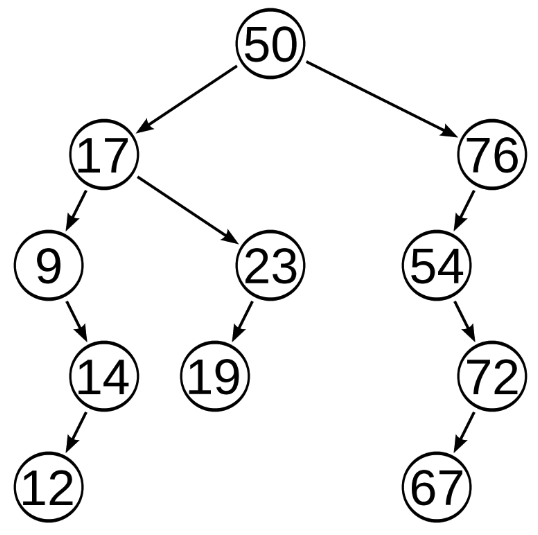
\includegraphics[width=0.95\textwidth]{tree.png}
                \end{center}
            \end{column}
        \end{columns}
    \end{frame}

    \begin{frame}
        \frametitle{Определения}
        \begin{itemize}
            \item Дерево --- совокупность элементов, называемых узлами (один из которых --- корень), и отношений, образующих иерархическую структуру узлов
            \begin{itemize}
                \item Узел является деревом, он же --- корень дерева
                \item Есть узел $n$ и деревья $T_1$, $T_2$, ..., $T_k$ --- деревья с корнями $n_1$, $n_2$, ..., $n_k$ соответственно. Тогда можно построить новое дерево, с корнем $n$ и поддеревьями $T_1$, $T_2$, ..., $T_k$. Узлы $n_1$, $n_2$, ..., $n_k$ называются сыновьями узла $n$
            \end{itemize}
            \item Нулевое дерево --- дерево без узлов
            \item Дерево --- связный ациклический граф
            \item Несвязный ациклический граф --- лес
        \end{itemize}
    \end{frame}

    \begin{frame}
        \frametitle{Ещё определения}
        \begin{itemize}
            \item Путь из $n_1$ в $n_k$ --- последовательность узлов $n_1$, ..., $n_k$, в которой каждый узел является родителем следующего
            \item Длина пути --- число, на единицу меньшее количества узлов, составляющих путь
            \item Путь нулевой длины --- путь из узла к самому себе
            \item Узел $a$ называется предком узла $b$, если существует путь из $a$ в $b$
            \begin{itemize}
                \item $b$ в этом случае --- потомок $a$
                \item Каждый узел --- предок и потомок самого себя
            \end{itemize}
            \item Потомок, не являющийся самим узлом, называется истинным потомком, с предком аналогично
            \item Узел, не имеющий истинных потомков, называется листом
            \item Поддерево какого-либо дерева --- узел вместе со всеми потомками
        \end{itemize}
    \end{frame}

    \begin{frame}
        \frametitle{И ещё определения}
        \begin{itemize}
            \item Высота узла --- длина самого длинного пути из узла до какого-либо листа
            \item Глубина узла --- длина пути от узла до корня
            \item Высота дерева --- высота корня
            \item Деревья бывают упорядоченными и неупорядоченными
            \begin{itemize}
                \item Можно упорядочить узлы дерева, не связанные отношением предок-потомок (слева-справа)
            \end{itemize}
            \item Деревья бывают помеченными (каждой вершине сопоставлено значение)
        \end{itemize}
    \end{frame}

    \begin{frame}
        \frametitle{Обходы}
        \begin{itemize}
            \item В глубину
            \begin{center}
                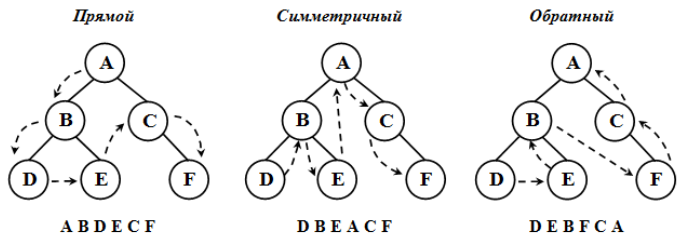
\includegraphics[width=0.8\textwidth]{dfs.png}
            \end{center}
            \item В ширину
            \begin{center}
                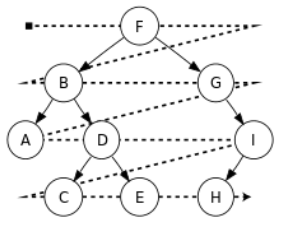
\includegraphics[width=0.25\textwidth]{bfs.png}
            \end{center}
        \end{itemize}
    \end{frame}

    \begin{frame}
        \frametitle{Деревья выражений}
        \begin{columns}
            \begin{column}{0.6\textwidth}
                $(a\,+\,b)\,*\,c\,+\,7$
                \begin{itemize}
                    \item Прямой порядок --- префиксная запись
                    \begin{itemize}
                        \item $+\,*\,+\,a\,b\,c\,7$
                    \end{itemize}
                    \item Обратный порядок --- постфиксная запись
                    \begin{itemize}
                        \item $a\,b\,+\,c\,*\,7\,+$
                    \end{itemize}
                    \item Симметричный порядок --- инфиксная запись
                    \begin{itemize}
                        \item $a\,+\,b\,*\,c\,+\,7$
                    \end{itemize}
                \end{itemize}
            \end{column}
            \begin{column}{0.4\textwidth}
                \begin{center}
                    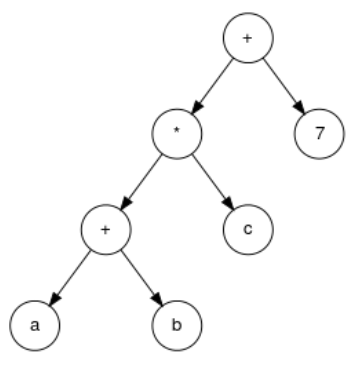
\includegraphics[width=0.8\textwidth]{expression-tree.png}
                \end{center}
            \end{column}
        \end{columns}
    \end{frame}

    \begin{frame}[fragile]
        \frametitle{АТД ``Дерево''}
        \begin{columns}
            \begin{column}{0.6\textwidth}
                \begin{itemize}
                    \item parent(n, t)
                    \item leftmostChild(n, t)
                    \item rightSibling(n, t)
                    \item label(n, t)
                    \item create(n, t1, ..., ti)
                    \item root(t)
                    \item makenull(t)
                \end{itemize}
            \end{column}
            \begin{column}{0.4\textwidth}
                \begin{footnotesize}
                    \begin{minted}{cpp}
void preorder(Node *n)
{
    printf("%s\n", label(n));
    Node *child = leftmostChild(n);
    while (child != NULL)
    {
        preorder(child);
        child = rightSibling(child);
    }
}
                    \end{minted}
                \end{footnotesize}
            \end{column}
        \end{columns}
    \end{frame}

    \begin{frame}[fragile]
        \frametitle{Нерекурсивный обход в прямом порядке}
        \begin{footnotesize}
            \begin{minted}{cpp}
void nonRecursivePreorder(Node *root) {
    Stack* stack = createStack();
    Node *current = root;
    while (true) {
        if (current != NULL) {
            printf("%s\n", label(current));
            push(stack, current);
            current = leftmostChild(current);
        } else {
            if (isEmpty(stack))
                return;
            current = rightSibling(top(stack));
            pop(stack);
        }
    }
    deleteStack(*stack);
}
            \end{minted}
        \end{footnotesize}
    \end{frame}

    \begin{frame}[fragile]
        \frametitle{Реализация списком сыновей}
        \begin{columns}
            \begin{column}{0.3\textwidth}
                \begin{footnotesize}
                    \begin{minted}{cpp}
struct Node
{
    ElementType value;
    struct Node *sibling;
    struct Node *child;
};
                    \end{minted}
                \end{footnotesize}
            \end{column}
            \begin{column}{0.7\textwidth}
                \begin{center}
                    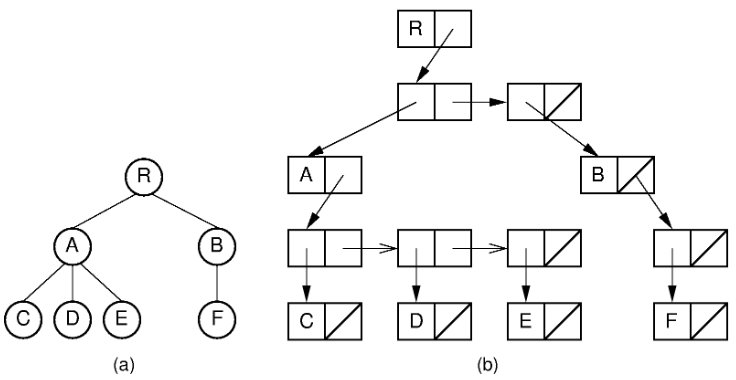
\includegraphics[width=0.8\textwidth]{children-list.png}
                \end{center}
            \end{column}
        \end{columns}
    \end{frame}

    \begin{frame}[fragile]
        \frametitle{Двоичные деревья}
        Деревья, у которых есть левый и правый сын, и это разные вещи
        \begin{columns}
            \begin{column}{0.4\textwidth}
                \begin{footnotesize}
                    \begin{minted}{cpp}
struct Node
{
    ElementType value;
    struct Node *leftChild;
    struct Node *rightChild;
};
                    \end{minted}
                \end{footnotesize}
            \end{column}
            \begin{column}{0.5\textwidth}
                \begin{center}
                    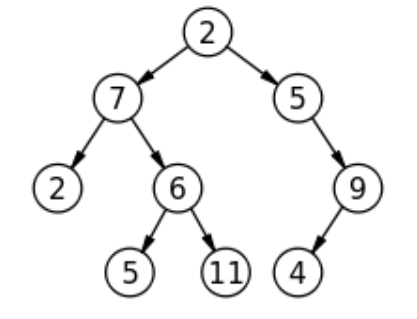
\includegraphics[width=0.8\textwidth]{binary-tree.png}
                \end{center}
            \end{column}
        \end{columns}
    \end{frame}

    \begin{frame}
        \frametitle{Пример: алгоритм Хаффмана}
        \begin{columns}
            \begin{column}{0.45\textwidth}
                \begin{itemize}
                    \item Алгоритм сжатия, вычисляющий кратчайшую кодовую последовательность для символа
                    \begin{itemize}
                        \item Если в тексте одни буквы ``А'', нет смысла кодировать А 16-ю битами
                    \end{itemize}
                    \item Префиксные коды
                    \item Дерево частот символов
                \end{itemize}
            \end{column}
            \begin{column}{0.55\textwidth}
                \begin{figure}[htp]
                    \centering
                    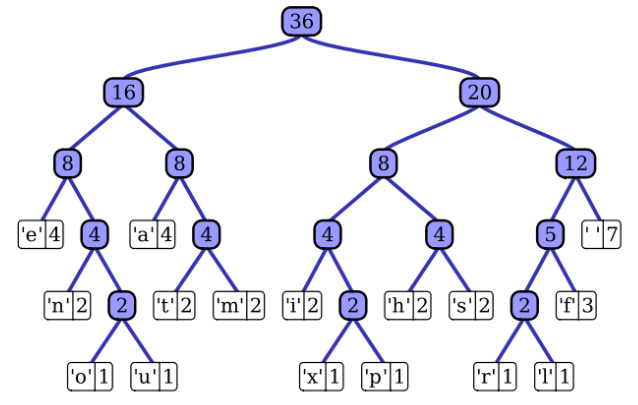
\includegraphics[width=0.8\textwidth]{huffman-tree.png}
                    Пример: ``this is an example of a huffman tree''
                \end{figure}
            \end{column}
        \end{columns}
    \end{frame}

    \begin{frame}
        \frametitle{Двоичное дерево поиска}
        \begin{columns}
            \begin{column}{0.6\textwidth}
                \begin{itemize}
                    \item Двоичное дерево, у которого для каждого узла в левом поддереве элементы, меньшие значения в узле, в правом --- элементы, большие значения в узле
                    \item Используется для представления множеств и ассоциативных массивов
                    \begin{itemize}
                        \item Если дерево сбалансировано (т.е. высота примерно логарифм количества вершин), операции вставки, удаления и поиска выполняются за $log(n)$
                    \end{itemize}
                \end{itemize}
            \end{column}
            \begin{column}{0.4\textwidth}
                \begin{center}
                    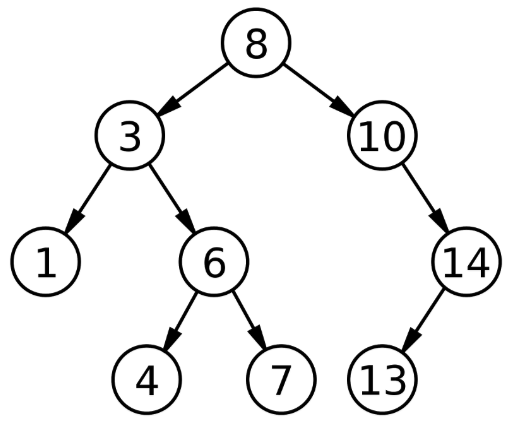
\includegraphics[width=0.8\textwidth]{bst.png}
                \end{center}
            \end{column}
        \end{columns}
    \end{frame}

    \begin{frame}
        \frametitle{Операции}
        \begin{itemize}
            \item Вставка
            \begin{center}
                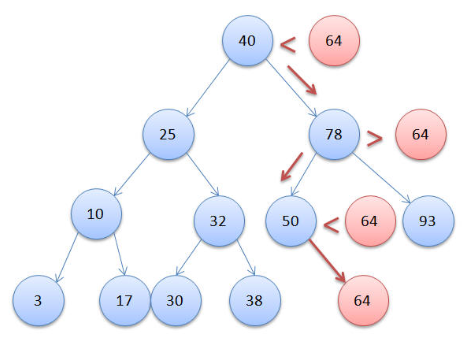
\includegraphics[width=0.4\textwidth]{insertion.png}
            \end{center}
            \item Удаление
            \begin{center}
                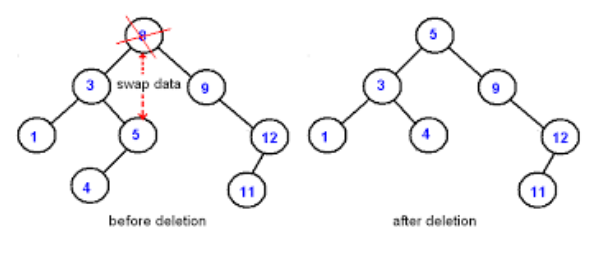
\includegraphics[width=0.5\textwidth]{deletion.png}
            \end{center}
        \end{itemize}
    \end{frame}

    \begin{frame}
        \frametitle{Проблема}
        \begin{itemize}
            \item При неудачном порядке вставки дерево может выродиться в список
            \item Трудоёмкости всех операций сразу станут линейными
        \end{itemize}
        \begin{center}
            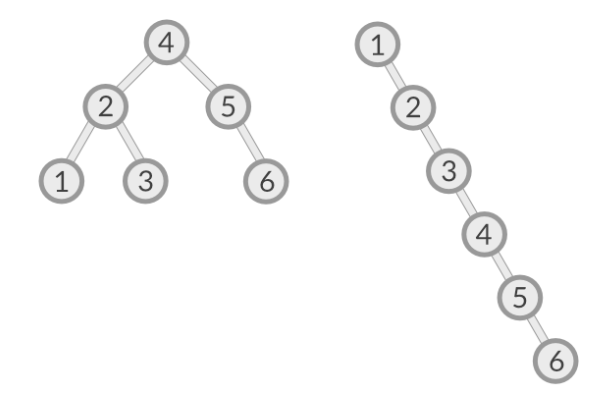
\includegraphics[width=0.5\textwidth]{problem.png}
        \end{center}
    \end{frame}

\end{document}